\subsection{Case Studies}
\label{sec:study}

The following case studies show how \lviz{} can be used to
understand system behavior and to solve system or application problems.
We first use a well understood task, file copying,
to familiarise the reader with \VDP{}.
We then use a software compilation example to show how \VDP{} can
be used for software failure diagnosis.
We use two visualizations on whole system traces to understand
how the operating system works and examine performance problems.
Lastly, we use \VDP{} to examine performance problems in a browser benchmark.
These examples also illustrate that the \VDP{} visualization is highly
customizable and in practice, one could use many different visualizations
on the same trace.

% In order to demonstrate the potential and power of visualizing system traces,
% we have developed a visualization tool \VDP{} using an extension of
% dotplots \cite{dnadp}.
% Dotplots were used to show sequence similarity in
% DNA \cite{dnadp} and music \cite{audio}.
% Our \VDP{} dotplots (or simply \VDP{} for both the visualization and tool)
% extends the basic dotplot to get a flexible visualization
% which can be tailored to visualize different kinds of behavior.
% Furthermore, \VDP{} uses a number of novel extensions geared towards
% understanding software behavior whereas traditional uses of dotplots
% are for showing sequence similarity.

The notation Bar $n$ refers to the $n$th barcode.
The configuration of each visualization is described in the corresponding
figure caption.

\subsubsection{Comparing File Copying Programs}
\label{sec:cp}

% \TODO{problems to solve: 1. finding repeated patterns
% 2. diagnose performance problem (8k buffer)}

% \begin{figure}[htb]
% \begin{center}
% 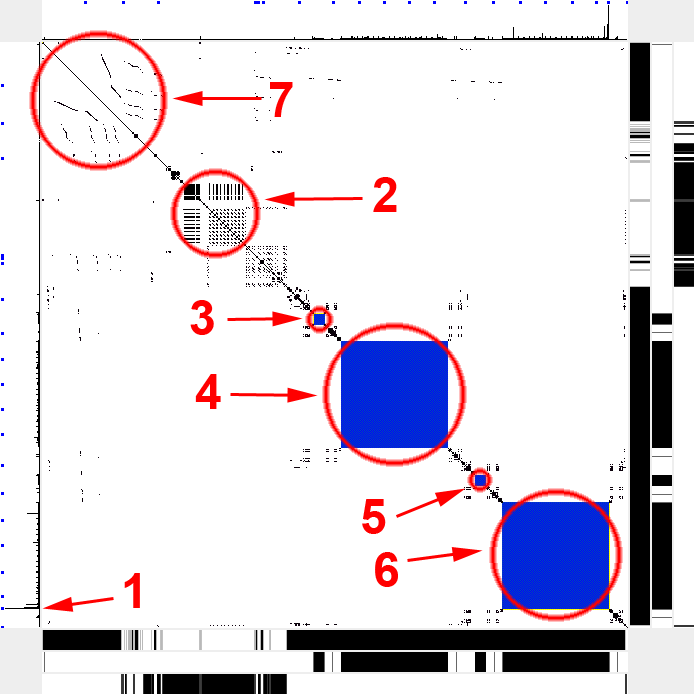
\includegraphics[width=1.0\columnwidth]{lviz/cp-xcopy.png}
% \caption{Self-comparison event-ordered \VDP{} of {\tt xcopy}
% copying 8 files of different sizes with the following configuration rules: 
% }
% \begin{tabular}{ll}
% DP match : & operation + parameter (pathname)\\
% DP color : & magenta $\rightarrow$ source; cyan $\rightarrow$ destination;\\
%  & black $\rightarrow$ other\\
% Bar1 color : & black $\rightarrow$ file operation\\
% Bar2 color : & black $\rightarrow$ source/destination files\\
% Bar3 color : & black $\rightarrow$ registry operation
% \end{tabular}
% \label{fig:cp-xcopy}
% \end{center}
% \end{figure}

\begin{figure}[htb]
\begin{center}

\includegraphics[width=0.10\columnwidth]{lviz/cp-zoom.png}
\caption{The alternate zoomed-in view of a blue region in
Fig.~\ref{fig:cp-xcopy} showing reading (magenta) and writing (cyan) operations.
}
\label{fig:cp-zoom}
\end{center}
\end{figure}

We use an example of a simple program and operation,
namely, file copying using \xcopy{}, to explain various
aspects of the \VDP{} visualization.
Fig.~\ref{fig:cp-xcopy} shows a self-comparison event-ordered \VDP{} of
\xcopy{} copying 8 files with sizes
1MB, 10KB, 10MB, 100KB, 1MB, 10KB, 10MB and 100KB and in that given order.
A self-comparison \VDP{} has a 45$^\circ$ diagonal line from top-left to 
bottom-right corner because events on the diagonal always match.
The structure of the files being copied is visible as blue squares in
Region {\em 3}, {\em 4}, {\em 5} and {\em 6} which show copying the
first 1MB and 10MB, then the second 1MB and 10MB files.
It is interesting to see the effect of scale on the visualization.
At this scale, which shows everything, the relative file sizes are also
visible for the large files.  The smaller 10KB and 100KB files are 
too small to be seen at this scale but are visible when zoomed in.
By correlating Bar1 and Bar2,
we find that there are some file related operations in the early phase,
but those files are neither source nor destination files of \xcopy{}.
This might seem surprising. To answer that question, we
click on Region 7, which shows that
the files in question are DLLs. Thus, the top-left region 
shows \xcopy{} loading DLLs.

Bar3 shows that Region {\em 2} has many registry operations which might
be surprising for a file copying task.
% This shows that a command line program can also have many
% registry operations.
The histogram spike at Region 1 shows that some events at the end of the
trace take a long time.
Fig.~\ref{fig:cp-zoom} is a zoomed-in view to one of the blue squares in
Fig.~\ref{fig:cp-xcopy}.
The checkerboard-like pattern shows alternating read (magenta) and write
(cyan) operations which is what we expect for file copy.
Since $cyan+magenta=blue$,
this explains that the blue squares in Fig.~\ref{fig:cp-xcopy} represents
reading from source files and writing to destination files.
We see also that visualizations at different scales can be used for
different purposes.
The extreme magnification in Fig.~\ref{fig:cp-zoom}
shows the actual operations but may be too detailed a view for
the overall picture which emerges at the other extreme in 
Fig.~\ref{fig:cp-xcopy}.

\begin{figure}[tbh]
\begin{center}
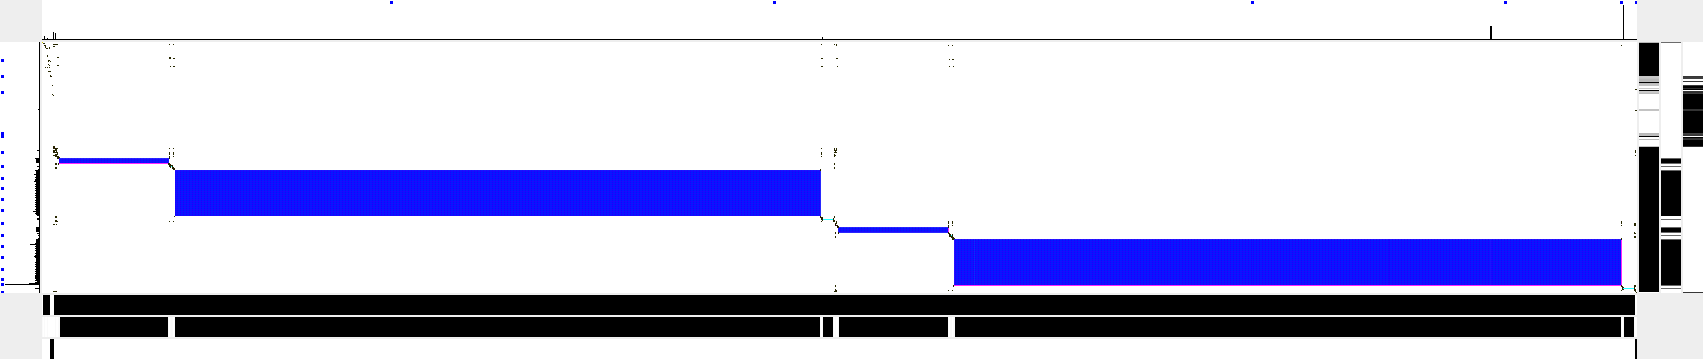
\includegraphics[width=1.0\columnwidth]{lviz/cp-xvc.png}
\caption{Event-ordered \VDP{} comparing {\tt cp} (x-axis) and {\tt xcopy} (y-axis) copying
the same files. 
The configurations are the same as in Fig.~\ref{fig:cp-xcopy}.
}
\label{fig:cp-xvc}
\end{center}
\end{figure}
%
\begin{figure}[htb]
\begin{center}
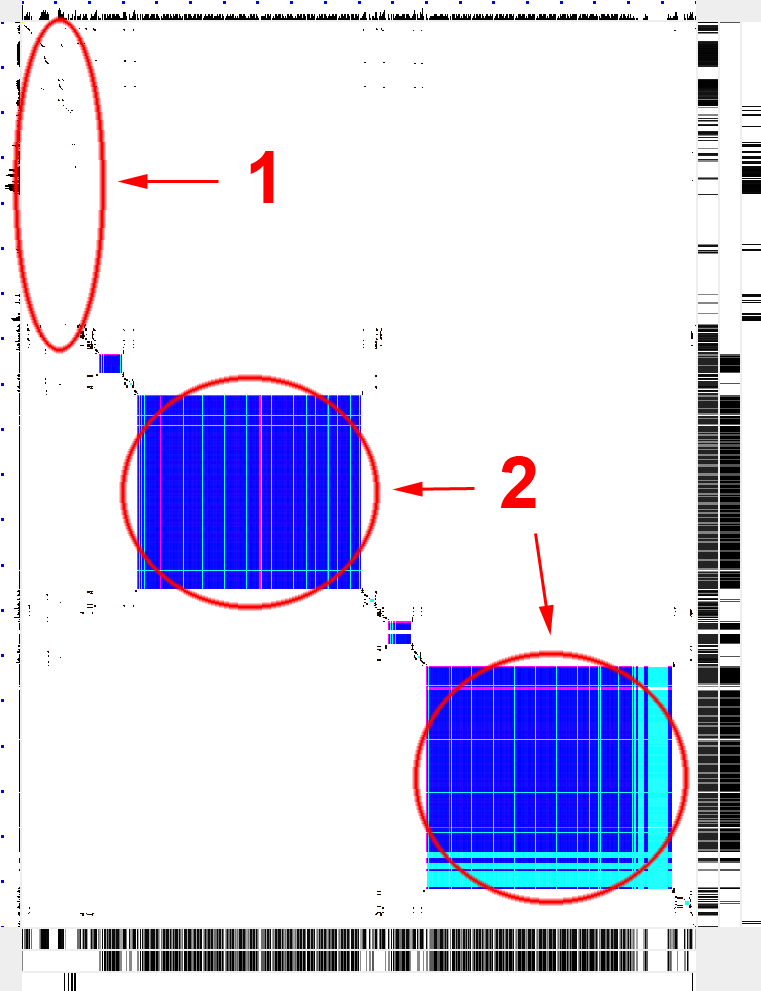
\includegraphics[width=0.6\columnwidth]{lviz/cp-64k.png}
\caption{Time-ordered \VDP{} comparing {\tt cp-64k} (x-axis)
and {\tt xcopy} (y-axis).
The configurations are the same as in Fig.~\ref{fig:cp-xcopy}.
}
\label{fig:cp-64k}
\end{center}
\end{figure}

In general, a \VDP{} is used with two traces rather than a single
trace as in a self-\VDP{}.
% Fig. \ref{fig:cp-xcopy} shows a \VDP{} which compares of a {\tt xcopy}
% trace against itself, i.e. a self-similarity comparison.
% Two different traces can also be compared with one trace on the X axis
% and the other trace on the y-axis.
Fig.~\ref{fig:cp-xvc} compares {\tt cp} (x-axis: a Windows version
of GNU {\tt cp}) and {\tt xcopy} (y-axis) copying the same 8 files.
% {\tt cp} is the Windows version of the file copying program included
% in GNU coreutils.
The \VDP{} is much wider than its height, giving
wide blue rectangles instead of blue squares 
(Fig.~\ref{fig:cp-xvc} versus Fig.~\ref{fig:cp-xcopy}).
% \TODO{double check width:height, shouldnt it be 16x?}
% Measuring the width and height of the rectangle,
% we find the ratio of width to height is approximately ? times.
Thus, {\tt cp} performs many more operations than {\tt xcopy}.
To investigate further, zooming in and examining individual events, 
we find that each read and write operation uses a buffer size of 4K,
while {\tt xcopy} uses 64K.
This means that {\tt cp} has 16 times more read and write operations
than {\tt xcopy}.
This is consistent with the width-height ratio in the visualization.

% \begin{figure}[htb]
% \begin{center}
% \includegraphics[width=1.0\columnwidth]{cp-xvct.png}
% \caption{Same as Fig.~\ref{fig:cp-xvc} but the axises are in time units.}
% \label{fig:cp-xvct}
% \end{center}
% \end{figure}

In order to compare the performance of {\tt cp} and {\tt xcopy},
we can use a time-ordered \VDP{}.
% In time based \VDP{}, events are distributed on the axises based on their
% relative time to the first event, while in event based \VDP{}
% events are distributed uniformaly.
Changing the visualization to a time-ordered one (not shown)
shows that {\tt cp} runs slower than {\tt xcopy} though less than 16x.
We then modified {\tt cp} to obtain another version
{\tt cp-64k} which uses 64K buffers.
Fig.~\ref{fig:cp-64k} shows the time-ordered \VDP{} comparing
{\tt cp-64k} (x-axis) and {\tt xcopy} (y-axis).
From Region {\em 2}, we can see that copying of the largest file
is performed in about the same time in both programs.
However, {\tt xcopy} has a slow initialization 
(as shown in Fig.~\ref{fig:cp-64k} Region {\em 1} which includes the registry
operations in Fig.~\ref{fig:cp-xcopy} Region {\em 2}),
which causes {\tt xcopy} to be slower in total than {\tt cp-64k}.

% \TODO{discuss flexible configuration and exploration process also shown
% in the other case studies}



\subsubsection{A Software Build Case Study}
\label{sec:build}

\begin{figure}[htb]
\begin{center}
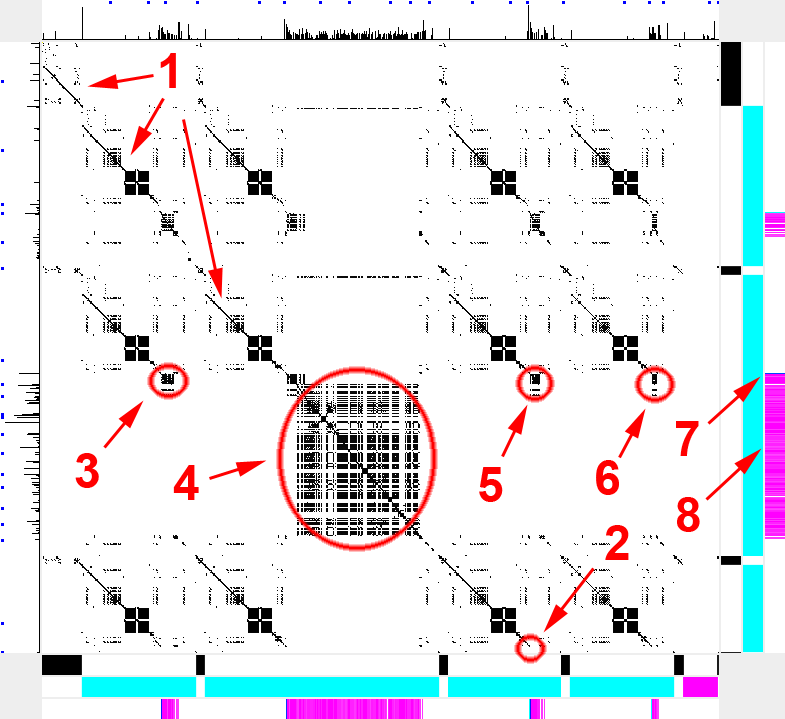
\includegraphics[width=1.0\columnwidth]{lviz/make-fail.png}
\caption{Event-ordered \VDP{} comparing a successful (x-axis)
software build process and a failed (y-axis) one.
%DP matching: program, operation and value (pathname);
%DP color: any=black;
%Bar1: {\tt nmake.exe}=black;
%Bar2: {\tt cl.exe}=cyan, {\tt link.exe}=magenta;
%Bar3: reading {\tt .c}/{\tt .h} files = cyan/magenta.
\label{fig:make-fail}
}
\begin{tabular}{ll}
DP match : & program + operation + value (pathname)\\
DP color : & black $\rightarrow$ any\\
Bar1 color : & black $\rightarrow$ {\tt nmake.exe}\\
Bar2 color : & cyan $\rightarrow$ {\tt cl.exe}; magenta $\rightarrow$ {\tt link.exe}\\
Bar3 color : & cyan $\rightarrow$ reading {\tt .c} files;\\
 & magenta $\rightarrow$ reading {\tt .h} files
\end{tabular}
\end{center}
\end{figure}

\begin{figure*}[htb]
\begin{center}
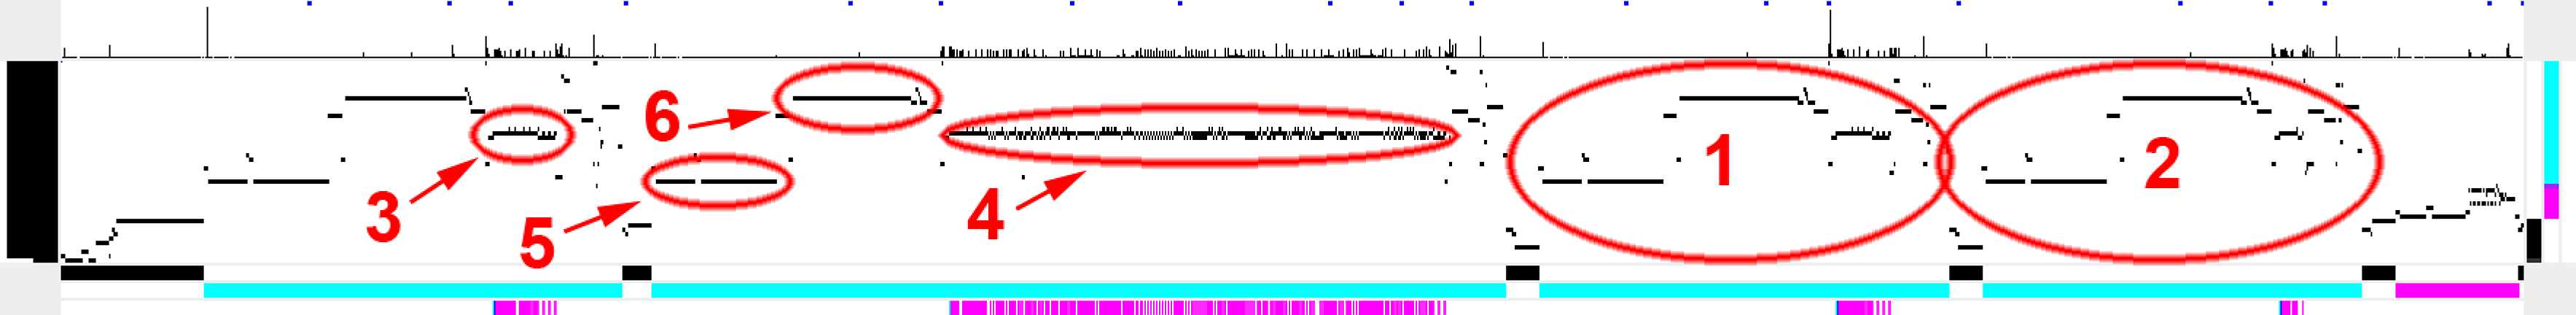
\includegraphics[width=1.0\textwidth]{lviz/make-pp.png}
\caption{Program point event-ordered \VDP{} of project build: pseudo program point trace (y-axis).
}
DP match: program name + program point;
DP color: black $\rightarrow$ any;
Barcode coloring rules are the same as in Fig.~\ref{fig:make-fail};
Bar3 in y-axis is undefined as the pseudo trace does not have operation type.
\label{fig:make-pp}
\end{center}
\end{figure*}

We now apply visualization to diagnose program failure.
In Fig.~\ref{fig:make-fail}, we compare a successful software project build
with a failed one to explain the failure.
The project consists of 4 C files, a header file and a {\tt makefile}.
We use {\tt nmake.exe} from Visual Studio to build the project.
To deliberately cause failure, one of the C files is changed
to be unreadable.

% Before identifying the cause of the failure,
We first explain what the visualization shows.
From the Bar2 of x-axis, 
we can see 4 {\tt cl.exe} processes (4 cyan regions), which tallies
with the number of C files.
There is one invocation of {\tt link.exe} (magenta),
occurring at the end of the trace.
By correlating Bar2 and Bar3, we see that
{\tt cl.exe} processes first read a C file (tiny blue bar in region {\em 7})
and then read a number of header files (long magenta bar in region {\em 8}).
Different {\tt cl.exe} processes read a different number of header files,
see sizes of regions {\em 3}, {\em 4}, {\em 5}, {\em 6} differ.

In a self-comparison \VDP{}, there will be a 45$^\circ$
diagonal line from top-left to bottom-right corner.
% The diagonal line means that the events
% on both x-axis and y-axis match (which is obviously true for self-comparison).
Fig.~\ref{fig:make-fail} shows a 45$^\circ$ diagonal (Label {\em 1})
with some breaks, from
the start to region {\em 2}, near the end of the failed build (y-axis).
It shows that the traces are basically similar till the failure point
when the build terminates.
By zooming in (not shown),
we see that the failure occurs at the third invocation of
{\tt cl.exe}, just before reading the C file.
Thus, the \VDP{} shows how file I/O works in the build and we use this
to identify a failed build.
One might argue that the compiler's error message is a better solution.
However, firstly,
not all software give detailed error message like the compiler in this case.
Secondly, due to software bugs, the error message could be wrong, while 
the system trace reports the actual underlying issues.

The build example is reused to show a visualization of the code structure
of {\tt cl.exe} in Fig.~\ref{fig:make-pp}.
We use a pseudo trace (y-axis) consisting of the program name
concatenated with its program point in the binary (an instruction address)
which is sorted by program name and address.
The program point comes from the stack walk corresponding to the event
and corresponds to the latest return address in the stack trace
coming from the executable or earliest DLL.
The x-axis trace is as before in Fig.~\ref{fig:make-fail}.

Region {\em 1} and {\em 2} show two invocations of {\tt cl.exe}
having similar patterns.
In fact, all 4 invocations follow the same pattern which can be broken
up into three main components:
region {\em 5}, {\em 6} and {\em 4}.
By zooming in and looking at the events, we infer that
region {\em 5} and {\em 6} is in the initialization phase of the compiler, which include
loading of DLL files and reading configurations from the registry.
Region {\em 6} is the reading of a large DLL {\tt rsaenh.dll}.
By looking at Bar3,
region {\em 3} and {\em 4} are the reading of C and header files.
As different C files have different header includes,
region {\em 3} and {\em 4} have different widths.
The fine squiggles in region {\em 3} and {\em 4} represent
three different file operations: open, read and close.
For each header file, there is one file open and close event,
with a differing number of file read operations depending
on the file size.
This makes the squiggles irregular.
Since this \VDP{} is based on program points, it shows directly the 
structure of the function calls. Thus, it visualizes
the code while Fig.~\ref{fig:make-fail} compares the operations
due to system calls.
It is also different from the source code visualization in \cite{tralfamadore}
and we do not need to rely on availability of source code.

The configurations play an important role in a \VDP{}.
Fig.~\ref{fig:make-matching} shows two \VDPs{} 
which are visually different from each other and also Fig.~\ref{fig:make-fail}
but they are all visualizations of the same underlying trace.
The \VDPs{} in Fig.~\ref{fig:make-matching} and 
Fig.~\ref{fig:make-fail} only differ in the DP matching rule and
the rest of the configuration is the same.
% The rest of the configuration and the two traces are exactly the same.
The left side \VDP{} in Fig.~\ref{fig:make-matching} uses only the event 
operation as the DP matching rule.
It can be used to highlight same or different operations.
The right side \VDP{} uses the program name, and can be used to
show different programs used in the project build process.

\begin{figure}[htb]
\begin{center}
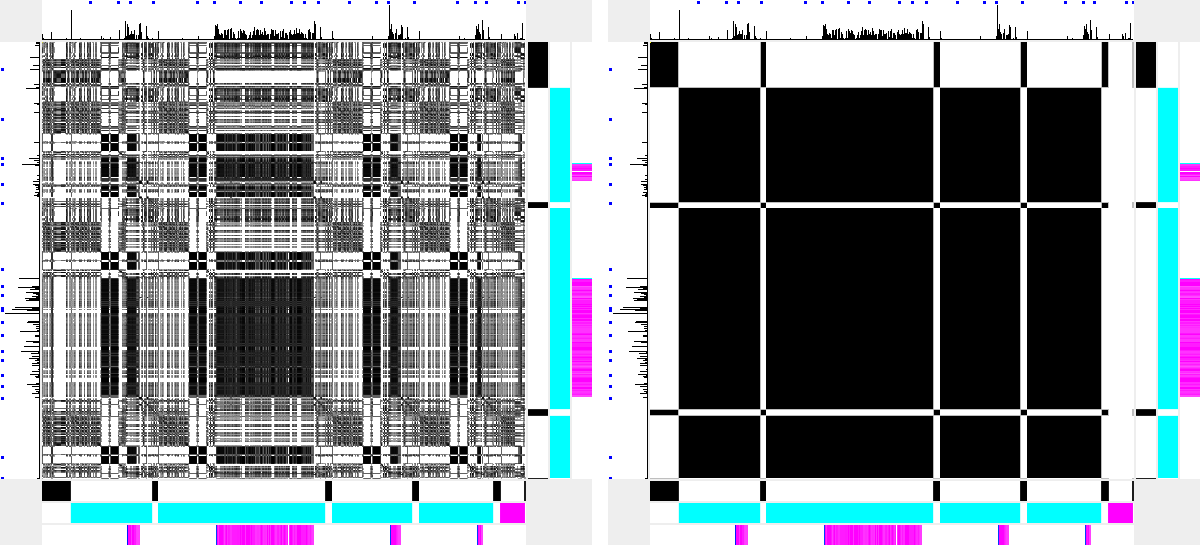
\includegraphics[width=1.0\columnwidth]{lviz/make-matching.png}
\caption{Changing the DP matching rule of Fig.~\ref{fig:make-fail}.
Left side DP matching rule is operation; Right side is program name.
}
\label{fig:make-matching}
\end{center}
\end{figure}

\TODO{reviewer 2:
In the second example, figure 8, a similar question: how do I know that a cyan bar is cl.exe and not some other
process - as a user I mean, not reading the legend of the figure? But the main question I have is why would a user go
to this level of effort to find why a build failed, he can always use the compiler's build log to find much more precisely
and more quickly what happened.
fixed.
}

\subsection{Visualizing Idle System Traces}
\label{sec:idle}

\begin{figure*}[htb]
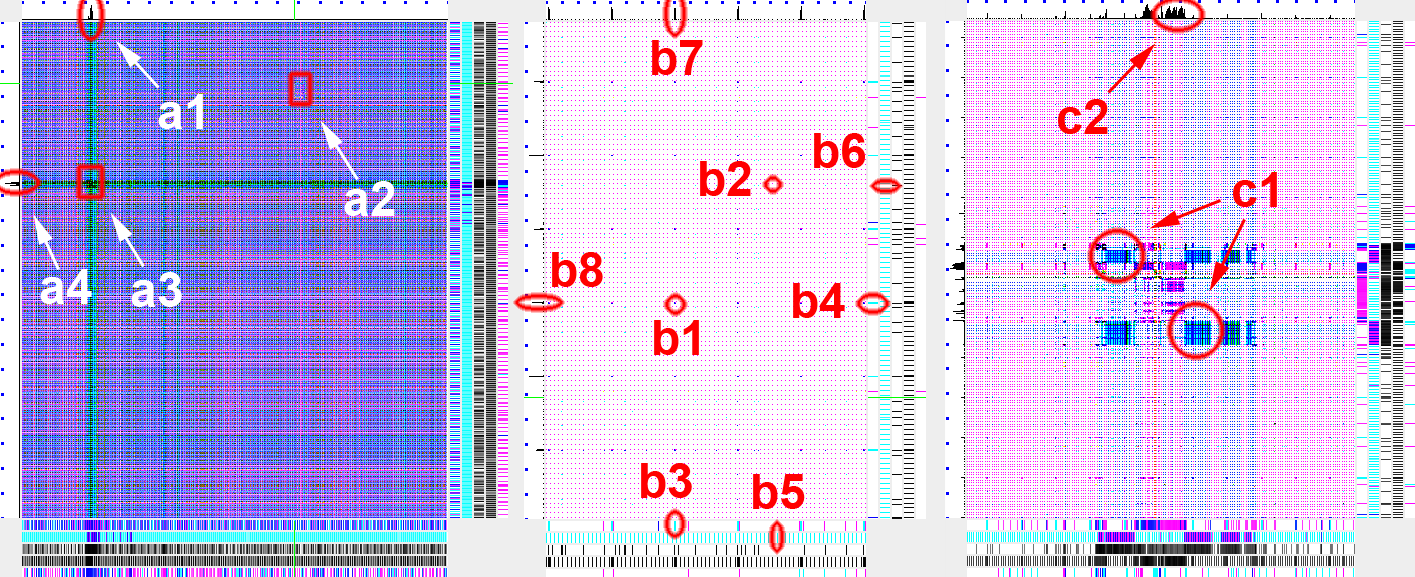
\includegraphics[width=1.0\textwidth]{lviz/idle-dp.png}
\caption{Time-ordered \VDP{} comparing two idle systems.
{\bf a.} (left) comparing one hour interval between two machines;
{\bf b.} (middle) zoom in of Region {\em a2};
{\bf c.} (right) zoom in of {\em a3}.
%DP Matching: (program,operation);
%DP color: file=cyan, registry=magenta, other operation=yellow;
%Bar1: lsass.exe=cyan, svchost.exe=magenta;
%Bar2: explorer.exe=cyan, wuauclt.exe=magenta;
%Bar3: file=black;
%Bar4: registry=black;
%Bar5: network=cyan, process\&thread creation\&termination=magenta.
The different DP color intensity in the zoomed views is caused by
histogram equalization.
}
\label{fig:idle-dp}
% \begin{tabular}{ll}
% DP match : & program + operation\\
% DP color : & cyan $\rightarrow$ file; magenta $\rightarrow$ registry; yellow $\rightarrow$ others\\
% Bar1 color : & cyan $\rightarrow$ lsass.exe; magenta $\rightarrow$ svchost.exe\\
% Bar2 color : & cyan $\rightarrow$ explorer.exe; magenta $\rightarrow$ wuauclt.exe\\
% Bar3 color : & black $\rightarrow$ file\\
% Bar4 color : & black $\rightarrow$ registry\\
% Bar5 color : & cyan $\rightarrow$ network, magenta $\rightarrow$ process \& thread creation \& termination
% \end{tabular}
{\it DP match}: program + operation;
{\it DP color}: cyan $\rightarrow$ file; magenta $\rightarrow$ registry; yellow $\rightarrow$ others;
{\it Bar1 color}: cyan $\rightarrow$ lsass.exe; magenta $\rightarrow$ svchost.exe;
{\it Bar2 color}: cyan $\rightarrow$ explorer.exe; magenta $\rightarrow$ wuauclt.exe;
{\it Bar3 color}: black $\rightarrow$ file;
{\it Bar4 color}: black $\rightarrow$ registry;
{\it Bar5 color}: cyan $\rightarrow$ network, magenta $\rightarrow$ process \& thread creation \& termination.
\end{figure*}


Previous examples compared the trace of particular programs
% against another
% so that we can compare the behavior of the two programs
(or to understand
how a program behaves using a self-similarity \VDP{}).
We now show that visualization can also be useful for system traces
as a whole -- a system trace is the complete trace of the entire operating
system for a period of time.

% \TODO{what is the problem}

When Windows is idle (i.e. no user interaction), 
system services and system processes still run.
We want to visualize whether such services and programs have 
(some expected) periodic behavior.
Fig.~\ref{fig:idle-dp}a (left) shows a time-ordered \VDP{} from two 
different idle machines for an hour at different times.
The size of the x and y-axis traces are 
851528 and 652713 events respectively.
% \footnote{
% Our \VDP{} tool handles large traces with real-time interaction.
% }
The configuration is described in the figure caption.
Bar1 and Bar2 show which events belong to
the four most active programs:
{\tt lsass.exe} is the Local Security Authority Subsystem Service which
enforces security;
{\tt svchost.exe} runs various services;
{\tt explorer.exe} is the graphical shell;
and {\tt wuauclt.exe} is windows auto-update service.
Bar3, Bar4 and Bar5 show the operation types.

Fig.~\ref{fig:idle-dp} shows periodic structure which appears
fractal-like.
Bar1 and Bar2 in Fig.~\ref{fig:idle-dp}a
show that events from {\tt lsass.exe}, {\tt svchost.exe} and {\tt explorer.exe}
occur continuously in the traces but {\tt wuauclt.exe} only occurs
during a short period of time.
Since this is time-ordering and the trace is one hour, we can conclude that
{\tt wuauclt.exe} occurs for about 7 minutes. (Bar2's magenta region
spans about 2
ticks in the histogram and there are 20 ticks in total.)
During this short period, we can see that a lot of events occur,
because the histogram at Region {\em a1} and {\em a4} have peaks.
We select two obvious regions to study the structure:
Region {\em a2} which is zoomed in Fig.~\ref{fig:idle-dp}b and 
Region {\em a3} zoomed in Fig.~\ref{fig:idle-dp}c.

We turn to the zoom in Fig.~\ref{fig:idle-dp}b.
Bar1 and Bar2 in
Fig.~\ref{fig:idle-dp}b show more clearly that
{\tt explorer.exe} (Region {\em b5} and {\em b6}) runs
more frequently than {\tt lsass.exe} (Region {\em b4} and {\em b3}).
Thus, we see two kinds of periodic events. The numerous dots such
as Region {\em b2} are the more frequent periodic events from 
{\tt explorer.exe} while the darker and less frequent dots such as
Region {\em b1} come from {\tt lsass.exe}.
Although {\tt explorer.exe} runs more frequently,
the event frequency histogram at Region {\em b7} and {\em b8} shows
that {\tt lsass.exe} has more events each time, hence Region {\em b1}
is darker than {\em b2}.
The white portions and together with the histogram show that there
are no other events in these portions of the idle trace.
% This means the load of {\tt explorer.exe} is spread out while
% the load of {\tt lsass.exe} is concentrated.

We have covered the periodic events in Fig.~\ref{fig:idle-dp}a except
for Region {\em a3}.
To explain Region {\em a3} and its zoom in Fig.~\ref{fig:idle-dp}c, 
we notice the cyan in Bar5 (network events) shows more activity.
Selecting those network events we find the
program is {\tt wuauclt.exe} (Windows update) --
both machines run Windows update at different time points explaining
the increase in network events.
% Selecting events in \VDP{} shows that the events are associated
% with {\tt wuauclt.exe} (Windows update) -- thus, it is Windows update
% running at a different point of time in both traces.
The dark Region {\em c1} shows that many of the events are the same 
in both machines in Windows update.
These events are file read and write to
{\tt C:\BS windows\BS softwaredistribution\BS datastore\BS datastore.edb}
(the Windows update database).
% We also see that network activity (outermost barcode) is higher in 
% Region {\em c3} during Windows update.
Other bursts of events in Region {\em c2} are generated by
{\tt svchost.exe} (it runs various Windows services) 
which operates on registry keys related to
windows installation.
% possibly due to the windows update.

This example shows that different machines not synchronized to 
each other have common periodic patterns and behavior.
We note that as we used idle traces, the frequency
of events will be low and a direct visualization is quite
faint. As such, \VDP{} employs equalization on the image 
to make the low frequency events more visible.

\TODO{reviewer 2:
In the example in 5.3, I understand that the task is to compare the behavior of Windows running idle on two different
machines. The question I have then is why would you use a 2D plot, when several histograms, stacked atop of each
other, could give you the same insight? That is, why is time ordering important here? I get the impression that the
same question holds for the system boot use case.
}

\subsection{System Boot}
\label{sec:boot}

\begin{figure*}[htb]
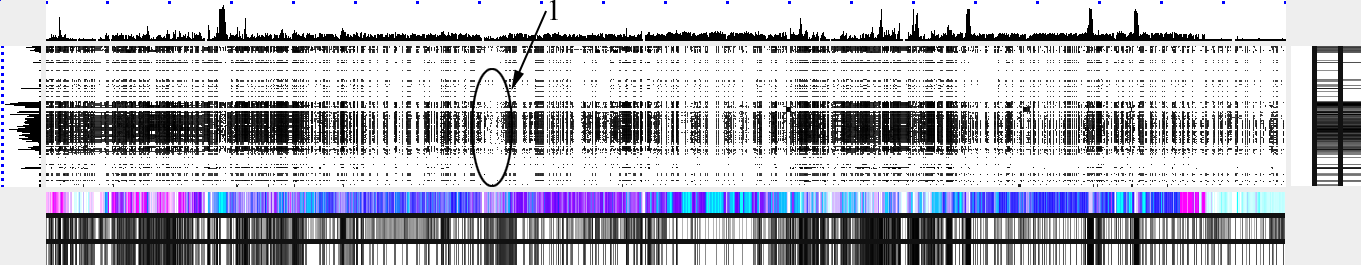
\includegraphics[width=1.0\textwidth]{lviz/boot-dp.png}
\caption{Time-ordered \VDP{} comparing boot
of a clean (Y axis) and a dirty (X axis) system.
}
\label{fig:boot-dp}
%\begin{tabular}{ll}
%DP match : & program + operation + parameter\\
%DP color : & black $\rightarrow$ any\\
%Bar1 color : & cyan $\rightarrow$ Google Desktop; magenta $\rightarrow$ AVG\\
%Bar2 color : & black $\rightarrow$ any program except Google Desktop and AVG\\
%Bar3 color : & black $\rightarrow$ file operation on Windows system directories\\
%\end{tabular}
{\it DP match}: program + operation + parameter;
{\it DP color}: black $\rightarrow$ any;
{\it Bar1 color}: cyan $\rightarrow$ Google Desktop; magenta $\rightarrow$ AVG;
{\it Bar2 color}: black $\rightarrow$ any program except Google Desktop and AVG;
{\it Bar3 color}: black $\rightarrow$ file operation on Windows system directories.
\end{figure*}

In Fig.~\ref{fig:boot-dp}, we use \lviz{} to investigate system boot and try to identify possible
factors causing a system to boot slowly.
To do this, we use a time-ordered \VDP{} to
compare a clean system which is known to boot quickly
with a (dirty) system which has many programs installed and boots slowly.

We see that the clean system boots much faster than the dirty system 
as the height is much shorter than the width.
Whenever Bar2 on the x-axis is not black,
the AVG (AVG antivirus) or Google Desktop is responsible for events.
We see that most of the events in the dirty boot are due to AVG or Google
Desktop.
We can also see from comparing Bar2 with Bar3
that the dirty system has other installed programs running
which are not in Windows directories.
%By looking at Bar1, we can clearly see that Google Desktop and AVG comprise about 5\% of boot time.

Even ignoring other programs outside the Windows directories,
the slowdown is also due to extra work by programs in Windows
directories.
We can see that this because some of the white DP gaps match up with 
black portions in Bar2 (program from Windows directory), e.g. Region 1.
This can be caused by the modification of the Windows system
by third party programs,
e.g. installing new services which are running in svchost.exe, and adding new registry keys or files
which will be scanned by windows programs.
To find out the details, we can focus on Windows built-in programs which
are identified by Bar3.
Vertical gaps in the Windows built-in program region identify the additional work done
by the Windows built-in programs in the dirty system.
By clicking in Region 1, we found out that the gap is caused by
{\tt svchost} (the generic processes for services) since
the new software installed uses {\tt svchost} to run some services.

%\input{lviz/ex-install}
\subsubsection{Web Browser Benchmark}
\label{sec:wbbench}

\begin{figure}[htb]
\begin{center}
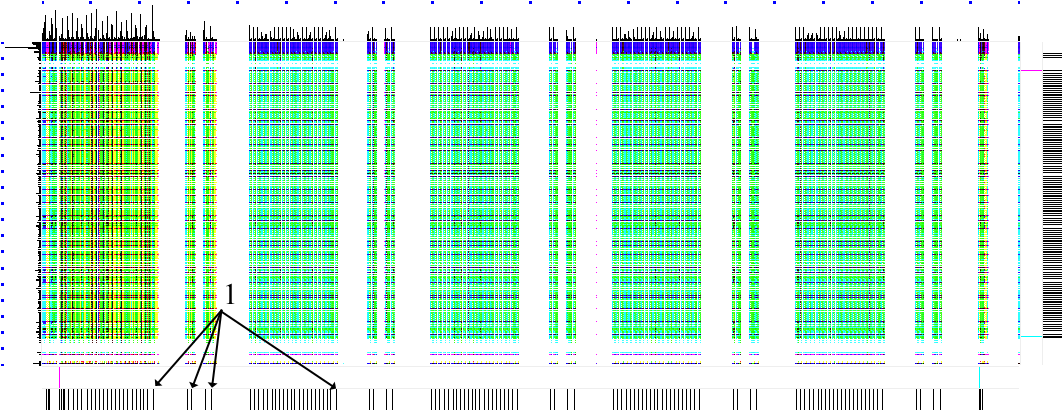
\includegraphics[width=0.7\textwidth]{lviz/wbbench-dp.png}
\end{center}
\caption{Time-ordered VDP comparing IE7 (x-axis) and Chrome (y-axis)
performing the
SunSpider JavaScript benchmark.
}
\label{fig:wbbench-dp}
%\begin{tabular}{ll}
%DP match : & operation\\
%DP color : & cyan $\rightarrow$ file; magenta $\rightarrow$ registry;
%yellow $\rightarrow$ network operation\\
%Bar1 color : & cyan $\rightarrow$ benchmark start time;
%magenta $\rightarrow$ benchmark end time\\
%Bar2 color : & black $\rightarrow$ HTTP GET event
%\end{tabular}
{\it DP match}: operation;
{\it DP color}: cyan $\rightarrow$ file; magenta $\rightarrow$ registry;
yellow $\rightarrow$ network operation;
{\it Bar1 color}: cyan $\rightarrow$ benchmark start time;
magenta $\rightarrow$ benchmark end time;
{\it Bar2 color}: black $\rightarrow$ HTTP GET event.
\end{figure}

We use time-ordered VDP (Figure~\ref{fig:wbbench-dp}) to investigate the
SunSpider JavaScript benchmarks on
two web browsers, Internet Explorer 7 (IE7) and Google Chrome.
The benchmark consists of 26 different tests repeated for 5 times.
Since the browser fetches a web page for each test,
we use the HTTP GET\footnote{
To mark HTTP GET events, we need to turn on network data I/O collection
and use a suitable regular expression as the barcode coloring rule.
The start and end events are marked by matching the two URLs.
}
event (shown in Bar2) to mark the beginning
of each test.
By looking at the time-ordered DP, we know that Chrome is about three
times faster than IE7 in total and also in each test.
From Bar2,
we can also observe that some tests (followed by long white gap,
pointed by marker 1) take much longer time than others.
By clicking on those events, we found out the slow ones to be all string
operation\footnote{
The URLs are \url{/perf/sunspider-0.9/string-base64.html},
\url{/perf/sunspider-0.9/string-tagcloud.html},
and \url{/perf/sunspider-0.9/string-validate-input.html}}
benchmarks.
We conclude that one reason why IE7 is slower than Chrome is due to string operations.

%\input{lviz/ex-iexploit}
%\input{lviz/ex-virus}
